\documentclass[12pt]{article}

\usepackage[a4paper,hmargin={2.4cm,2.4cm},vmargin={2.4cm,2.4cm}]{geometry}
\usepackage[mathlines,displaymath]{lineno}
\usepackage{setspace}
\usepackage{amsmath}
\usepackage{amsfonts}
\usepackage{bm}
\usepackage{graphicx}
\usepackage[round,colon,authoryear]{natbib}
\usepackage{color, soul}
\usepackage{fancyvrb}
\usepackage{verbatim}
\usepackage[pdftex,colorlinks=true,citecolor=black,linkcolor=black,urlcolor=black,pdftex,pdfstartview=FitH,bookmarks=true]{hyperref}
\usepackage{rotating}

\bibliographystyle{ecology}



\begin{document}

\title{Improved state-space models for inference about spatial and
  temporal variation in abundance from count data}

\author{Richard B. Chandler  \\
        \small USGS Patuxent Wildlife Research Center \\
        \small Laurel, MD 20708
   \and Jeffrey A. Hostetler \footnote{Contact:
     \url{HostetlerJ@si.edu}, +001-202-633-4205}\\
%        \small Migratory Bird Center \\
        \small Smithsonian Conservation Biology Institute \\
        \small National Zoological Park, MRC 5503 \\
        \small Washington, DC 20013-7012}
\maketitle


\abstract{
Models of population dynamics play a central role in theoretical and
applied ecology where they are used for purposes such as testing
hypotheses about density dependence and predicting species' responses
to future environmental change or conservation actions. Accounting for
process variation and observation error in such efforts is necessary
to achieve unbiasedness \hl{[may be too strange sounding a term for
  abstract]}, and doing so is possible using recently
developed state-space models.
%for estimators of population change to be unbiased, and state-space
%models have been developed for this
%models are widely used for these purposes because they allow for
%estimating parameters of classical growth models, such as exponential,
%logistic, and Gompertz, while accounting for demographic stochasticity
%and observation error.
Conventional state-space models, however, have
three important limitations: (1) the parameters are not identifiable
in many common situations, (2) they do not admit spatial variation in
population dynamics, and (3) there is no clear interpretation of the
observation error. We demonstrate how each of these problems can be
resolved using a class of hierarchical models for spatially-replicated
time-series data recently proposed by \citet[Biometrics]{dail_madsen:2011}.
We expand this class of models to accommodate classical growth
models, zero-inflation, and random effects such as observer-specific
detection probabilities. We also present methods for forecasting
population size under future environmental conditions. Implementation
of these ideas is possible using either frequentist or Bayesian
methods, and code to fit these models using the  \textbf{R} package
\texttt{unmarked} or
\textbf{JAGS} is also provided.
%is provided for doing so.
%Furthermore, we describe classical and
%Bayesian methods of parameter estimation, and we present methods of
%forecasting population size under future environmental
%conditions.
%These new developments will
%allow researchers to apply these methods to address important
%questions regarding the factors affecting spatial and temporal
%variation in abundance.
A simulation study indicated that bias was negligible and coverage nominal
and an analysis of North American Breeding Bird Survey is presented
for illustration.
}

\vspace{0.5cm}

\textbf{Key words}: abundance, Dail and Madsen model, density-dependence,
Gompertz model, immigration, open population point count models,
random observer effects, range, Ricker model, zero-inflated

\newpage

Theoretical ecology requires models of population dynamics for testing
hypotheses regarding spatial and temporal variation in
abundance. For example, much theoretical work has focused on
understanding the importance and existence of phenomenon such as
density-dependent population regulation, population cycling, and spatial synchrony
\citep{may:1975,royama:1977,turchin:1990,dennis_taper:1994,bjornstad_etal:1999},
and population models are required to evaluate associated hypotheses.
In applied contexts, population models are used for
estimating extinction probabilities
\citep{schoener_spiller:1992,nadeem_lele:2011} and for predicting the
effects of future environmental conditions or conservation actions on
population size \citep{jamieson_brooks:2004,hatfield_etal:2012}.
In order to address these questions, two complicating factors must
be confronted when fitting population models to data.
First, deterministic models of population
dynamics are virtually always inadequate due to process variation,
the inherent stochasticity in demographic parameters and environmental
conditions \citep{bjornstad_grenfell:2001,saether_engen:2002}.
Second, abundance---the natural state variable in studies
of population dynamics---can rarely be observed perfectly in field
studies because of observation error, such as imperfect
detection \citep{link_nichols:1994,kery_etal:2009}.

State-space models are a widely used approach for
studying population dynamics while accounting for process variation
and observation error \citep{devalpine_hastings:2002,
  buckland_etal:2004, dennis_etal:2006}. Classical state-space
models are time-series models in which the true state of the
system (e.g. population size during each year) is observed
imperfectly. One reason for the widespread adoption of state-space
models in ecology is that failure to account for process variation and
observation error can bias estimators of abundance and population
growth parameters. For instance, the strength of
density dependence will be over-estimated if observation error is
ignored \citep{link_nichols:1994,shenk_etal:1998}.

A simple state-space models can be described as follows.
Let $N_t$ be the abundance of a species during year $t$, for
$t=1,\hdots,T$, and let $X_t$ be
the observed data, which differs from $N_t$ due to observation error,
a random effect denoted $\zeta_t$. Temporal variation in $N_t$ is
modeled using a population growth model, $\mu(N_{t-1})$,
coupled with a stochastic model allowing
for random process variation. %, which we denote $\grave{o}_t$.
The deterministic model may be density-dependent, for example
logistic, or it might be density-independent, as in the case of
exponential growth, in which $\mu(N_{t-1}) = N_{t-1}e^{r}$ where $r$
is the intrinsic rate of increase. The full model can now be written
as:
\begin{subequations}
  \label{eq:ss1}
  \begin{align}
    N_1 &= X_1 \label{eq:ss1a} \\
    N_t &= \mu(N_{t-1}) + \grave{o}_{t-1} \quad \text{for} \; t=2,\hdots,T \label{eq:ss1b} \\
    X_t &= N_t + \zeta_t \qquad \qquad \;\, \text{for} \; t=1,\hdots,T \label{eq:ss1c}
  \end{align}
\end{subequations}
where $\grave{o}_t$ is the random effect allowing for process
variation unaccounted for by the deterministic model. In classical
state-space models, the two sets of random effects
are assumed to be i.i.d Gaussian deviates:
$\grave{o}_t \sim \mathrm{N}(0, \sigma)$ and
$\zeta_t \sim \mathrm{N}(0, \tau)$. It is also standard practice to
ignore process variation associated with $N_1$, as
indicated by Eq~\ref{eq:ss1a}.

Even though state-space models such as that shown in Eq.~\ref{eq:ss1}
are the most widespread approach for modeling population dynamics
using time-series data, several problems are evident. Namely, (1)
time-series data and the underlying abundance parameters of interest
are typically integer-valued, as in the case of count data, raising
concerns about the use of Gaussian distribution for the random
effects, (2) the model for observation error has little biological basis, (3)
spatial variation in abundance is not allowed, and (4) some of the
paramters of the model are not estimable. We briefly discuss each of
these points before describing a general approach to resolving these
shortcomings.

Use of the Gaussian distribution for modeling random process variation
and observation error is motivated by convenience rather than
biology. Specifically, the Gaussian assumptions
allow for parameter estimation using the Kalman filter
\citep{dennis_etal:2006}, which is much more computationally efficient
than estimation methods when random effects are not Gaussian distributed
\citep{devalpine_hastings:2002}. The problem with this is that it
allows for negative values of the state-variable, which is
inconsistent with the observed data.
%The fact that both abundance ($N_t$) and the observed data ($X_t$) are
%typically non-negative integers suggests that it is inappropriate to
%model process variation and observation error using Gaussian
%distributions.
Nonetheless, efforts have been made to adhere to the
Gaussian assumptions by tranforming abundance to
density by replacing $N_t$ with $Y_t = \log(N_t/A)$ where $A$ is the
area surveyed. However, this transformation is problematic since
local abundance may be zero and thus $Y_t = \log(0) = -\infty$. Generally,
zeros are replaced with some small number, although the
effect of this is rarely discussed.

Another problem with standard state-space models is that the
observation error has no clear interpretation. The use of a mean zero
Gaussian distribution implies that $X_t$ will be
higher than $N_t$ as often as it is lower than $N_t$. It is hard
to identify a mechanism that would cause such symmetric errors. A more likely
form of observation error, and one that has been recognized for well
over a century, results from failing to detect individuals that are
present. Imperfect detection may be attributable to
characteristics of the species under study, such as its elusiveness,
or to the failings of the ecologist collecting the data in the field.
Although a vast number of methods have been devised for accounting for
this form of observation error, rarely have these methods been
integrated into state-space models \citep[but
see][]{buckland_etal:2004}.

A more serious problem than the ones associated with the Gaussian
assumptions is that the parameters of the simple state-space models
such as Eq~\ref{eq:ss1} are not identifiable in many
circumstances \citep{polansky_etal:2009}. Recall that the
Eq.~\ref{eq:ss1} did not specify distributions for $N_1$; % or $X_1$;
however, $N_1$ is a random variable and hence there is uncertainty
that should be accounted for.
%are needed to fully specify the model.
To be more specific, a fully-specified state-space model requires at least
three probability distributions, which we represent
using bracket notation: \hl{[I'm not familiar with bracket notation,
  so these equations are confusing to me.  How widely used is this
  notation in ecology?  Will others likely understand this?]}
\begin{subequations}
  \label{eq:ss2}
  \begin{align}
    [N_1&|\bm{\theta}] \\ \label{eq:ss2b}
    [N_t&|N_{t-1},\bm{\Theta}] \quad \text{for} \; t=2,\hdots,T \\ \label{eq:ss2c}
    [X_t&|N_t,\bm{p}]  \qquad \; \text{for} \; t=1,\hdots,T
  \end{align}
\end{subequations}
where $\bm{\theta}$ are the process variation parameters for the
initial state, $\bm{\Theta}$ are the process variation parameters
influencing how abundance changes over time, and $\bm{p}$ are the
observation error parameters. The three lines of general model
described by Eq.~\ref{eq:ss2} correspond to the three equations shown
for the specific example in Eq~\ref{eq:ss1}.  However, in this case,
we allow $N_1$ to be a random variable. But what should its
distribution, $[N_1|\bm{\theta}]$ be? And how could $\bm{\theta}$ be
estimated since there is only a single observation available?
One approach to estimating the $\bm{\theta}$ is to assume that the
population is in equlibrium, i.e. that the expected value of $N_t$ is
constant through time. Althought this makes the parameters
identifiable, assuming equlibrium defeats the objective of many
studies of population dynamics, namely determining why a population
varies over time.

\begin{comment}
  However, a completSpecifically, the Markovian nature of the model
  implies the following likelihood The first term is the probability
  density for the first observation in the time series, $X_1$, yet it
  is intuitively not possible to estimate the parameter(s) of this
  distribution using only a single observation.
  % This problem has resulted in several papers with interesting names
  % like ``multi-modal likelihoods and ridges etc...''
  Two options have been proposed handling the identifiability
  problem. First, one can assume that the first observation in the
  time series is made without error. Second, one can assume that the
  population is at equilibrium so that that the x can be replaced with
  the equilibrium distribution. However, assuming equilibrium defeats
  the objective of many studies of population dynamics, namely
  determining if and why a population is at equilibrium.
\end{comment}

A fourth problem with these models is that they do not admit
spatial variation. This reduces the scope of the inferences that can
be drawn from the models and it ignores the importance of space in
population regulation.
%, which
%restrict the utility of their since it is typically
%impossible assess the impacts of factors such as habitat
%fragmentation or climate change on population dynamics without
%considering spatial variation in abundance. Indeed many populations are
%regulated by spatial processes such as source-sink dynamics.

Several extensions of state-space models have been proposed to
overcome the limitations described
above. \citet{devalpine_hastings:2002} and \citet{kery_etal:2009}
described methods for fitting models with non-Gaussian distributions
for the process and observation errors. Observation models with more
intuitive interpretations, such as those that explicitly model
detection probability, have been proposed by
\citet{kery_etal:2009}. \citet{lele_etal:1998} and
\citet{kery_etal:2009} developed models allowing for inference about
spatial and temporal variation in abundance, and their developments
also resolved the problems of non-identifiability for the parameters
of the initial state at time $t=1$. Of these extensions, the work by
\citet{kery_etal:2009} is unique in that it addressed multiple limitations
simultaneously. However, their model did not include serial
dependence, which is a hallmark of population models. This limits the
utility of their model for making inferences about explicit population
processes. In contrast, recent work has sought to use state-space
models for inference about population processes such as mortality and
recruitment. To do so, methods have been developed to combine multiple
sources of information, such as counts and mark-recapture data
\citep{besbeas_etal:2002, buckland_etal:2004,
  schaub_etal:2007}. Although these integrated
population models may be viewed as the gold standard in state-space
modeling, ecologists are not always so fortunate to have direct
information about vital rates, especially at large spatial scales.
Rather, count data are much more common, and
are produced by many of the largest monitoring programs in the world,
such as the North American Breeding Bird Survey
\citep[BBS;][]{robbins_etal:1986}.

In this paper, we focus on the model of
\citet[henceforth the DM model;]{dail_madsen:2011}
%developed a model (henceforth the DM model)
that simultaneous resolves each of the abovementioned problems with
traditional state-space models, and is designed for simple count
data.
\begin{comment}
  The model (1) recognizes
  the discrete nature of count data and the underlying true abundance
  state, (2) includes a realistic observation model with explicit
  detection probability parameters (3) has estimable parameters,
  including those describing the initial state at time $t=1$, and (4)
  allows for inference about both temporal and spatial variation in
  abundance.

  In some respects, the DM model can be viewed as a specific
  manifestation of the general state-space model formulated by
  \citep{buckland_etal:2004}. However, their model was designed to
  allow for inference about demographic parameters, which will
  typically require mark-recapture data. Although this may be viewed
  as the gold standard in many studies of wildlife populations, in
  this paper, we focus on the analysis of count data, which is the
  typical source of information used in state-state modeling
  applications, and one of the most widely available forms of
  ecological data---it is also the data required by the DM model.
\end{comment}
In the following section, we describe the DM model in its original
form and explain how it resolves each of the deficiencies with
standard state-space models. In Section~\ref{sec:ext}, we extend the
model to accomodate classical models of population growth and to
handle several features common to ecological
time-series. Specifically, we describe methods for accomodating excess
zeros and nuisance variables such as random observer effects. Both
frequentist and Bayesian methods of inference are discussed, and code
for fitting models is presented in the appendices.
%The Bayesian method
%is attractive in that it can accomodate prior information about
%detection parameters, which is available for many species, yet not
%collected as part of many existing monitoring programs.
In Section~\ref{sec:app}, we evaluate the performance of the model
extensions using a simulation study and by analyzing data from the
North American Breeding Bird Survey (BBS), one of
the most spatially and temporally extensive sets of count data on
vertebrate populations \citep{robbins_etal:1986}. The overarching aim
of  the paper is to provide ecologists with flexible and accessible means of
adressing important questions related to the variation of abundance in
space and time.
%believe these extensions will increase the utility of the model for
%application to existing datasets such the Breeding Bird Survey.

\begin{comment}
  The DM model allows for inference about spatial and temporal
  dynamics in abundance while accounting for observation error using
  only spatially and temporally replicated count data.  Their model is
  an extension of the closed-population $N$-mixture model
  \citep{royle:2004biom}, which was designed specifically to address
  the problem of modeling spatial variation in abundance in the
  presence of observation error, specifically, when detection
  probability is less than one. The DM extension relaxes the
  assumption of population closure and includes explicit parameters
  describing population change as a first-order Markovian
  process. [more details]

  [applications / potential etc... ] The DM model is relevant to a
  vast number of problems confronting basic and applied ecological
  research. Answering questions about climate change etc... require
  spatially and temporally extensive datasets such as result from the
  North American Breeding Bird Survey (BBS)
  \citep{robbins_etal:1986}. However, most of the datasets of the
  appropriate scale are collected by volunteers and using protocols
  that are not amenable to traditional approaches of modeling
  abundance and detection probability based on standard
  capture-recapture methods. Instead they have, at best, simple count
  data for which, when it can be interpreted as counts of unique
  individuals, the DM model can be applied.. Yadi ya

  Although the DM model was designed explicitly for these purposes,
  the original formulation of the model makes strict distributional
  assumptions and does not acknowledge many of the sources of
  variation inherent to existing ecological time-series data.  We
  propose variations on these models that are likely to be more
  realistic and useful in many cases.  We demonstrate the usefulness
  of these new models with simulated and real BBS data.


  In this paper, we demonstrate how the DM model resolves each of
  these four limitations of conventional state-space models, and we
  extend the DM model in several important ways. First, we demonstrate
  how classical population models can be embedded within the DM
  model. Then we present methods for handling excess zeros as well as
  nuisance parameters such as random observer effects on detection
  probability. A simulation study
\end{comment}


\section{The Dail-Madsen Model}
\label{sec:dm}

The DM model is an extension of the $N$-mixture model
\citep{royle:2004biom}, which allows for inference about spatial
variation in abundance when individuals cannot be detected with
certainty. To estimate both abundance parameters and parameters of the
detection process, the original $N$-mixture model uses replicate
observations at each site, which are collected during sufficiently
short time intervals such that the population can safely be assumed to
be closed with respect to births, deaths, and movement. The DM model
relaxes this closure assumption and includes explicit parameters
describing population change over time.


\subsection{The Data}

The DM model requires count data collected at $R$ sites, each of which
is surveyed on $T$ time periods. A site is ideally, but not necessarily, a
well-defined region of a study area, such as a wetland or a patch of
early-successional habitat. In some cases, a site may not have a clear
biological significance, for instance in the case of randomly located
survey plots. The timeframe of the study is arbitrary, but the general
situation is one in which the time period is sufficiently long such
that abundance changes at each site. We will call
these time periods primary sampling periods to distinguish them from
secondary sampling periods, which are repeated surveys within a
primary period. In the case where no secondary sampling was conducted,
let $n_{it}: i=1,\hdots,R; t=1,\hdots,T$ denote the count data at site
$i$ and primary period $t$. If $J$ secondary sampling periods were used, $n_{ijt}:
j=1,\hdots,J$ is the count at site $i$ during secondary sampling
occasion $j$ within year $t$. These are the observed data, which
typically will less than the actual quantitiy of interest, abundance,
denoted $N_{it}$. In cases where detection probability is perfect,
abundance is observed directly such that $\{N_{it}\}$ are the data.

\subsection{The Model}

As originally formulated, the DM model includes submodels for three
conditionally related processes: (1) initial abundance, i.e. the
abundance at site $i$ during the first primary period,
denoted $[N_{i1}]$, (2) subsequent abundance, which is dependent upon
abundance in previous years $[N_{it}|N_{it-1}]$, and (3) the
detection process, $[n_{it}|N_{it}]$ \citep{dail_madsen:2011}.
The first two processes describe the state process---the
variation in abundance in space and time. The third item in the list
is the observation process, which describes the relationship between
the true state, abundance, and the observed count data.

\subsubsection{Initial abundance}

In the original formulation, initial abundance was
modeled using either the Poisson or negative binomial distributions:
\begin{gather}
N_{i1} \sim \mathrm{Pois}(\Lambda_i) \nonumber \\
\text{or} \nonumber \\
N_{i1} \sim \mathrm{NB}(\Lambda_i, \alpha)
\label{eq:N1}
\end{gather}
where
%$N_{i1}$ is the abundance at site $i=1,\hdots,R$ during year 1 and
$\Lambda_i$ is the expected abundance at site $i$ during year 1. The
Poisson distribution assumes that the mean of $N_{i1}$ is equal to its
variance, whereas the negative binomial distribution allows the
variance to be greater than the mean with the amount of overdispersion
determined by the parameter $\alpha$.

Regardless of the specified distribution, the model for initial
abundance has two distinguising features. First, it provides a
mechanism for characterizing spatial variation in abundance. For
instance, one might consider the influence of some environmental
covariate ($x_i$) on abundance using a log-linear
model such as $\log(\Lambda_i) = \beta^{\Lambda}_0 + \beta^{\Lambda}_1
x_{i}$. The second important point is that the spatial replicates resolve the
problem of parameter non-identifiability that are common to standard
state-space models because, as demonstrated by \citet{royle:2004biom},
process variation and observation error can be estimated from
spatially-replicated count data. Hence, the first component of the
model addresses issues (1) and (2) identified in the introduction.

\subsubsection{Abundance in subsequent time periods}

The DM model assumes that abundance in time $t$ is a function of
abundance in time $t-1$, i.e. abundance at each site evolves as a
first order Markovian process, although
higher order processes are also possible.  \citet{dail_madsen:2011}
considered several models to describe the temporal dynamics; however,
in each case they modeled $N_t$ as the sum of two random variables:
$S_t$, the number of indivduals surviving from $t-1$ and not
emigrating; and $G_t$ the number of new individuals entering the
population. Their most general model was
\begin{equation}
\left.\begin{aligned}
S_{it}|N_{it-1} &\sim \mathrm{Bin}(N_{it-1}, \omega) \\
G_{it}|N_{it-1} &\sim \mathrm{Pois}(\gamma(N_{it-1})) \\
N_{it} &= S_{it}+G_{it}
\end{aligned}\right\} \quad \text{for} \; t=2,\hdots,T
\label{eq:Nt}
\end{equation}
where $\omega$ is the apparent survival probability and $\gamma$ is
the recruitment rate (which can depend on $N_{it-1}$). In the absence
of movement, $\omega$ is exactly the probability of surviving from
year $t$ to $t-1$, and $\gamma$ is the per-capita birth rate. However,
in the more common scenario when immigration and emigration occur,
$\omega$ is the probability of surviving and not emigrating, and
$\gamma$ is product of the birth rate and the emigration rate,
i.e. the recruitment rate. \citet{dail_madsen:2011} proposed three
models for $\gamma$: the constant model,
$G_t \sim \mathrm{Pois}(\gamma)$ where recruitment does not depend on
$N_{it-1}$, and which simulates a ``propagule rain'' of new individuals; the
autoregressive model, $G_t \sim \mathrm{Pois}(\gamma(N_{it-1}))$, which
simulates geometric or density independent growth; and the
``no-trend'' model, $\gamma = (1-\omega)\Lambda$, which keeps
expected abundance constant over time. As before, covariates of
$\omega$ and $\gamma$ can be easily accomodated, for example using
logit- and log-linear models respectively.

In cases where no movement occurs, the DM model can directly estimate
demographich parameters, and this mechanistic description of
population change is much more appealing than classical
population growth models such as the logistic model. However, movement
complicates the interpretation of the the parameters, reducing the
connection to specific population processes. In such cases, the model
of dynamics shown in Eq~\ref{eq:Nt} can be replaced with standard
population models as described in Sect~\ref{sec:ext}. Irrespective of
the model for population dynamics, it is worthwhile to note that the
discrete distributions used in the DM model avoid the issues
associated with the Gaussian distribution used to model process
variation in standard state-space models.

\subsubsection{Observation process}

Eqs.~\ref{eq:N1} and \ref{eq:Nt} fully specify the state model---the
model for spatial and temporal variation in abundance. The observation
model assumes that individuals are missed due to imperfect
detection. The simplest model for imperfect detection is
\begin{equation}
  n_{it} \sim \mathrm{Bin}(N_{it}, p)
  \label{eq:p1}
\end{equation}
Surprsingly detection probability, $p$, can be estimated without
secondary sampling occasions. However, this is only possible because
if the parameteric assumptions of the population dynamics are met
exactly. In practice, it is preferable to obtain direct information
about $p$ using secondary sampling occassions or some other auxiliary
data, as is demonstrated in section


\section{Statistical Inference}

\subsection{Maximum likelihood}

Maximum likelihood estimation of parameters in models with random
effects requires removing the random effects by integration or
summation.



\subsection{Bayesian inference}

Bayesian inference has several appealing features. First, it allows
direct probability statements to be made about a hypothesis given
data. Second, priors are cool. We can combine data from multiple
sources or use existing estimates of parameters as prior
distributions. MCMC has a bad rap for being slow, but actually, in the
case of state-space models it may be one of the few options for
estimation, and in fact may be faster than maximizing likelihoods.

Here is some BUGS code:
\begin{verbatim}
model {
lambda ~ dunif(0, 5)
r ~ dunif(-5, 5)
p ~ dunif(0,1)
for(i in 1:nSites) {
  N[i,1] ~ dpois(lambda)
  y[i,1] ~ dbin(p, N[i,1])
  for(t in 2:nYears) {
    mu[i,t-1] = N[i,t-1]*exp(r)
    N[i,t] ~ dpois(mu[i,t-1])
    n[i,t] ~ dbin(p, N[i,1])
    }
  }
}
\end{verbatim}



\section{Model Extensions}
\label{sec:ext}

\subsection{Population growth models}

Preliminary DM model runs for several species tended to lead to
estimates of survival that were unrealistically high and recruitment
that were unrealistically low, or the reverse (compared to independent
demographic analyses).  The DM models are able to partition changes in
abundance to survival and recruitment in part by making strong
distributional assumptions. % (Dail and Madsen 2011).
When those assumptions are heavily violated the models may proportion
population growth incorrectly into survival and recruitment, even if
they estimates population growth accurately.

Although partitioning population growth into survival and recruitment
is informative, it is not needed for all applications.  Furthermore, a
simpler model would have several merits: faster running time, fewer
total model combinations, and possibly more realistic estimates.
Therefore, we developed a version of the DM model that estimates and
models population growth directly.  In this model, Eq.~\ref{eq:Nt} is
simplified to:
\begin{equation}
  N_{it} \sim \text{Pois}(\exp(r)N_{it-1})
\label{eq:exp}
\end{equation}
where $r$ represents the instantaneous population growth rate.  This,
like the autoregressive version of the model, is a variant on a simple
density-independent exponential model of population growth.
Density-dependent versions of the model are also possible.  For
example:
\begin{equation}
  N_{it} \sim \text{Pois}(N_{it-1}\exp(r(1-N_{it-1}/K))
\label{eq:rick}
\end{equation}
where $K$ is the stable equilibrium of the population and $r$ is the
instantaneous population growth rate at low population densities, and
both parameters are constrained to be positive.  This model is based
on the \citet{ricker:1954} discrete time version of the logistic population
growth model.  We also implemented the \citet{gompertz:1825} density-dependent
model:
\begin{equation}
  N_{it} \sim \text{Pois}(N_{it-1}\exp(r(1-\log(N_{it-1})/\log(K)))
\label{eq:gomp}
\end{equation}
where the log of $N_{it-1}$ is only taken when $N_{it-1}>0$
(when $N_{it-1} \equiv 0$, the full expression simplifies to 0 anyway).  Here
the interpretations of $r$ and $K$ are similar to in the Ricker model, but
$K$ is constrained to be greater than one.

Because a single Poisson distribution controls the
distribution of $N_{it}$ in each of these models, the discrete
convolution used by \citet{dail_madsen:2011} is not required,
speeding up processing time.

\subsection{Immigration models}

The autoregressive, population growth, Ricker, and Gompertz
versions of the DM models all share a common feature (or bug):
once the population at a site reaches 0, it must remain at 0.
This is because all contributions to population growth are
local in these models.  We generalized each these models that
include both internal and external (immigration) contributions
to population growth.  The population growth plus immigration
model is:
\begin{equation}
  N_{it} \sim \text{Poisson}(\exp(r)N_{it-1}) + \text{Poisson}(\iota)
  \label{eq:expimm1}
\end{equation}
or equivalently
\begin{equation}
  N_{it} \sim \text{Poisson}(\exp(r)N_{it-1} + \iota)
  \label{eq:expimm2}
\end{equation}
where $\iota$ represents the immigration rate.  This model is close to
the constant DM model (equation 4), with $\exp(r)$ instead of $\omega$
and $\iota$ instead of $\gamma$, except that the first
process is Poisson distributed instead of binomial. The Ricker and
Gompertz models can be extended to allow for immigration in the same
way.
\begin{comment}
  Similarly, the Ricker + immigration model can be represented as: the
  Gompertz + immigration model as: (13) and the autoregressive +
  immigration model as: (14)
\end{comment}

% Save for discussion
\begin{comment}
  These immigration models are based on the assumption that number of
  immigrant is not dependent on local density; however, extending
  these models in this way is conceptually straight-forward, a Other
  versions of these models with different assumptions are
  possible. The Ricker + immigration and Gompertz + immigration models
  can be justified by the further assumption that immigrants arrive as
  adults immediately before the point-count survey (so that
  density-dependent processes do not have a chance to act on the
  numbers of immigrants; Otto and Day 2007 p. 161).  Deterministic
  versions of these models do reach stable equilibriums, but the
  equilibriums are not at K and cannot be solved for analytically
  (Otto and Day 2007).
\end{comment}

We have implemented all preceding models in
a maximum likelihood framework by extending the \texttt{unmarked} package
\citep{fiske_chandler:2011} in \textbf{R} \citep{R-2012}.


%\subsection{Range model of initial abundance}
\subsection{Excess zeros}

\citet{dail_madsen:2011} suggested two distributions for modeling
initial abundance: Poisson and negative binomial.  We have extended
their model to include another distribution, the zero-inflated
Poisson.  This could be useful when, for example, one is modeling the
abundance of several bird species with the same set of BBS routespoint
count surveys for all species, but this set includes routes sites
outside the range of some of the bird species.  The distribution of
initial abundances can be represented as:
\begin{equation}
N_{i1} \sim \left\{
\begin{aligned}
0 &\; \text{with probability} \; \psi \\
\Lambda &\; \text{with probability} \; (1-\psi)
\end{aligned} \right.
\label{eq:ZIP}
\end{equation}
where $\psi$ represents the proportion of extra zeros.

These models allow three sources of zero counts by observers: a
species was at a route but not detected; the route was within the
species' range but there were no birds at that site in that year; and
the route was outside the species' range.  Furthermore, detection,
abundance, and zero-inflation can be modeled separately as functions
of different (or the same) covariates.  For example, detection of
species x at site y in year z might depend on wind speed, abundance on
forest type and weather, and zero-inflation upon elevation and
climate.  This approach combines elements of occupancy modeling
\citep{mackenzie_etal:2006} and abundance modeling.
%, and could prove useful
%for distinguishing species' fundamental and realized niches
%(Hutchinson 1957).

The zero inflation factor can also affect
recruitment or population dynamics (see below).
We also considered a zero-inflated negative binomial model of initial
abundance, but this model did not perform well in preliminary tests.

%\subsection{Dynamic range models}

The zero-inflated Poisson distribution can be applied to not only
initial abundance but also to recruitment and population growth terms.
For example, the recruitment term of the constant DM model (equation
4) can be modified as follows:
\begin{equation}
G_{it} \sim \left\{
\begin{aligned}
0 &\; \text{with probability} \; \psi \\
\mathrm{Poisson}(\gamma) &\; \text{with probability} \; (1-\psi)
\end{aligned} \right.
\label{eq:ZIPts}
\end{equation}
When both initial abundance and dynamics are modeled as zero-inflated,
$\psi$ can be modeled as time-varying or not (in either case, $\psi$ can also be
modeled as varying over space).  In the latter case, it makes sense
for the model to "remember" which sites are inside the range of the
species between the initial abundance stage and each time step of the
dynamics stage (see code sample?).  Adding zero-inflation to the
dynamics of the autoregressive, trend, Ricker, or Gompertz models
(without immigration) should have no effect when initial abundance is
also zero-inflated unless $\psi$ is time-varying (because these dynamic
models cannot recover from zero abundance).  We have implemented
zero-inflated dynamics in the Bayesian framework using program
\textrm{JAGS} \citep[version 3.2.0]{plummer:2003}.
%(version 3.2.0; Plummer 2003)


\subsection{Random effects of observers}

Differences in observers' ability to see, hear, or identify
birds has long been recognized as a potential source of error
in avian point count surveys such as the BBS
\citep{robbins_etal:1986,diefenbach_etal:2003,sauer_etal:1994auk,alldredge_etal:2007auk,campbell_francis:2011}.
Estimating a separate detection probability for each observer can be
difficult and reduces one's ability to estimate the quantities
of interest.  This problem is compounded by the fact that
observers differ greatly in the number of surveys they have
run (so that many observers' separate detection probabilities
could not be accurately estimated).

Current BBS trend estimators deal with this problem by
treating observer identity as a random (as opposed to a fixed)
effect \citep{link_sauer:2002,sauer_link:2011}.
%(Link and Sauer 2002, Sauer and Link 2011).
This allows observer-specific differences in detection probability,
but assumes that observers are selected at random from a pool
of potential observers.  Models that contain both random and
fixed effects are referred to as mixed models.  Often in mixed
models (as in this case), the random effect is modeled not
because it of interest in itself, but to avoid bias in the
estimates of the fixed effects.

To include random observer effects in DM models and these extensions,
Eq.~\ref{eq:p1} can be modified to:
\begin{gather}
n_{ijt} \sim \mathrm{Bin}(N_{it}, p_j) \nonumber \\
\mathrm{logit}(p_j) \sim \mathrm{Normal}(\mu_p, \sigma_p)
\label{eq:pobs}
\end{gather}
where $n_{ijt}$ is the number of bird recorded at site $i$ by observer $j$ in
year $t$, $p_j$ is observer-specific detection probability, $\mu_p$ is the mean
detection probability (on the logit scale), and $\sigma_p$ is the standard
deviation of the random observer effects (also on the logit scale).
We have implemented random observer effects in the Bayesian framework
using program \textbf{JAGS} \citep[version 3.2.0]{plummer:2003}
% (version 3.2.0; Plummer 2003)
with the \textbf{R} (R
Development Core Team 2011) package \texttt{rjags} \citep{plummer:2011}
%(Plummer 2011)
interface.


\section{Forecasting Future Population Size}





\section{Applications}
\label{sec:app}

\subsection{Simulation Study}


We simulated data for 100 sites over 40 years.  All
simulations assumed initial abundance was Poisson distributed
and no covariates affected initial abundance, dynamics, or
detection probability.  Our first series of simulations
assumed dynamics were exponential.  We ran 1000 simulations for
each combination of low, medium, and high $\Lambda \in \{1,5,10\}$, $r
\in \{-0.005, 0, 0.005\}$, and
$p \in \{0.05, 0.25, 0.5\}$. % (Table 1; 27 total combinations).

Our second series of simulations changed dynamics to the
Ricker model.  We used an initial abundance of 10, a maximum
growth rate of 0.005, and a detection probability of 0.25, and
simulated low, medium, and high values of equilibrium
abundance, each with 500 simulations (Table 1).  Our third
series of simulations was based on the Ricker + immigration
dynamics model; here we fixed all parameters the same as the
Ricker model (with K = 10) and simulated low, medium, and high
values of immigration rate with 500 simulation each (Table
1).

We estimated the parameters for each simulation using the same
initial abundance (Poisson) and dynamics models as were
simulated, implemented in the unmarked library in \textbf{R}.  When run
in a maximum likelihood framework, these models require a
maximum abundance to integrate over
\citep{royle:2004biom,dail_madsen:2011};
%(Royle 2004, Dail and Madsen 2011);
we used 200.  We report bias of estimates, root
mean squared error, and coverage (percentage of 95\% confidence
intervals for parameters that
overlap the true values).

Ideas:
I.	Test importance of random effects modeling, and other differences between JAGS and unmarked
II.	Model with low p values, or a range of p values
III.	Ability to distinguish correct initial abundance and dynamics models
IV.	When can you detect DD if it exists (power)?
V.	Building on the last two: what if your model set doesn't
include the correct DD model?  When will the wrong DD model be favored
over the wrong DID model?



\subsection{Analysis of Breeding Bird Survey Data}

We applied these models to North American Breeding Bird Survey (BBS)
data from 1966-2010 for two species in the bordering US states
Maryland and Virginia.  For our focal species, we selected ovenbirds
(\textit{Seiurus aurocapilla}), an abundant and widespread forest breeding
migrant with a stable or increasing trend in the region (CITE) and
golden-winged warblers (\textit{Vermivora chrysoptera}), which only breeds in
the western parts of these states and has been declining in the region
(CITE).  MORE INFORMATION ABOUT THE SPECIES?

GENERAL ABOUT BBS DATA.  We only used data marked as acceptable for
use in the annual BBS analysis.  We summed the total birds of each
species seen on each route and year and used the routes (rather than
the individual stops) as our sites.
Strong winds can interfere with point count observers' ability to hear
birds (\citep{simons_etal:2007}); we tested the effects of wind speed
on detection probability.  BBS volunteers record wind conditions at
the beginning and end of each route on the Beaufort Scale
\citep[start and end wind 0-9]{robbins_etal:1986}.
%(start and end wind; Robbins et al. 1986)(start and end wind; 0-9; cite).
When
start or end wind was not recorded we imputed those values with the
start or end mean.  We took the mean of start and end wind for each
route and put this average wind scale value into four categories: 0 $\leq$
wind $<$ 1; 1 $\geq$ wind $<$ 2; 2 $\leq$ wind $<$ 3; and wind $\geq$ 3 (maximum of 3.5).
Following \citet{link_sauer:2002},
%Link and Sauer (2002),
we also included the first time an
observer ran a route as a predictor variable for detection
probability.

HOW WE OBTAINED AND MANIPULATED PRISM DATA
We ran a series of maximum-likelihood based models for each species,
and then a series of Bayesian models.  We started by testing three
models of initial abundance (Poisson, negative binomial, and
zero-inflated Poisson) with population growth dynamics (equation 7)
and no covariates.  We selected the minimum Akaike's Information
Criterion (AIC) model from that set to test three additional models
for p: wind, first, and wind + first.   We selected the minimum AIC
model from that set to test eight additional models of dynamics:
constant, autoregressive, Ricker, Gompertz, autoregressive +
immigration, population growth + immigration, Ricker + immigration,
and Gompertz + immigration.  We then tested the effect of average
minimum temperature for June and July on all dynamics parameters from
the minimum AIC dynamics model.  When run in a maximum likelihood
framework, these models require a maximum abundance to integrate over
(Royle 2004, Dail and Madsen 2011); we used 600 for ovenbirds and 350
for GWWA.

We ran the top ranked models from the maximum likelihood analyses in a
Bayesian framework.  We added random observer effects and, where
appropriate, zero-inflated dynamics.  WILL ADD MORE HEREWe used
non-informative priors.  We tested for lack of convergence using X
Markov chains for each model \citep{gelman_rubin:1992}.
%(Gelman and Rubin 1992).
For each chain
we sampled the MCMC for Y iterations, after Z tuning samples.  Latent
inclusion factors for temperature effects?

\section{Results}



The negative binomial distribution was strongly supported for ovenbird
initial abundance over the Poisson and zero-inflated Poisson (Table
1A, models A.1 - A.3).  Even compared to the Poisson, there was no
evidence to support a zero-inflation factor for this species.  The
best supported model for p was additive effects of wind speed and
first run (Table 1A, model A.4).  First run and increasing wind speeds
both decreased p.  All dynamics models with immigration were better
supported than models without immigration (Table 1A, models A.8 -
A.16); the best supported of these was the Ricker + Immigration.  The
best supported model of those without immigration was the Gompertz,
and the autoregressive and the constant model had the least support.
There was little support for an effect of minimum June and July
temperature on dynamics parameters of the Ricker + Immigration model
(Table 1A, models A.17 - A.18).

Estimates for the top ranked model for OVEN
(NB[$\Lambda (.) \alpha (.)$]Ricker+Imm.[$r(.)K(.) \iota (.)$]p(wind+1st)) were similar when
run in the Bayesian framework, except that the estimate of r more than
halved (from 0.026 $\pm$ 0.006 to 0.011 $\pm$ 0.005 [for Bayesian model
estimates we present mean and SD]).  When random observer effects were
added, estimates for $\Lambda$ and K increased dramatically (from 31.6 $\pm$ 4.9
to 42.5 $\pm$ 7.3 and from 56.2 $\pm$ 18.2 to 101.8 $\pm$ 21.1, respectively), and
the estimate for r was intermediate (0.018 $\pm$ 0.006).  The estimate of
the intercept for p (on the logit scale) dropped from -1.5 $\pm$ 0.1 to
-2.0 $\pm$ 0.1, and the estimate of $\sigma_p$ was 0.35 $\pm$ 0.03.  [Richard, I ran
the temperature model in the Bayesian framework (w/ and w/o random
effect) too.  Should we include those results?  As earlier, very
little evidence for an effect of temperature on any of the parameters,
although I couldn't get the latent inclusion parameter to work for r.]
Gelman and Rubin diagnostics and visual examination of the ? plots
provided some evidence for a lack of convergence in estimates of the
intercept for p for all Bayesian models ran.

There was slightly more support for the ZIP distribution for initial
abundance of GWWA than for the negative binomial; both were strongly
supported over the Poisson (Table 1B, models B.1 - B.3).  The best
supported model for p was an effect of first run (Table 1B, model
B.4).  The best supported dynamics model was population growth (Table
1B, model B.8); the estimate of r from this model was -0.058 $\pm$ 0.017
(SE).  There was no support for immigration added to the population
growth or autoregressive models (Table 1B, models B.10 and B.13).
However, the Gompertz + immigration and Ricker + immigration models
were supported over the corresponding models without immigration
(Table 1B, models B.11, B.12, B.14, and B.15), despite low estimates
of $\iota$ from these models (0.003 $\pm$ 0.003 and 0.003 $\pm$ 0.002,
respectively).  There was considerable support for an effect of
average minimum June and July temperature on r in the population
growth model (Table 1B, model B.17), with a negative slope.

Because of the closeness of rankings for the ZIP and negative binomial
distributions for GWWA, we also ran the subsequent models with the
negative binomial initial abundance.  Rankings of subsequent models
were similar, but with a p covariate (first) the negative binomial
distribution outranked the ZIP.

STILL WORKING ON JAGS GWWA RESULTS
Estimated detection probabilities were generally low.  For OVEN, the
estimated probability of detecting a bird with no wind and not the
first time an observer had run a route varied between 0.046 $\pm$ 0.002
(model A.16) and 0.192 $\pm$ 0.015 (model A.11), among models that
accounted for both.  For GWWA, the estimated probability of detecting
a bird by a non-first time observer varied between 0.025 $\pm$ 0.008
(model B.18) and 0.141 $\pm$ 0.027 (model B.16), among models that
accounted for first but not wind.

For both species, constant dynamics models estimated very high
survival probabilities ($\omega$ = 1 $\pm$ 1.3e-05 for OVEN and 0.935 $\pm$ 0.011 for
GWWA).   The autoregressive and autoregressive + immigration models
estimated very low survival probabilities for OVEN ($\omega$ = 0.058 $\pm$ 0.046
and 0.026 $\pm$ 0.060, respectively), but not for GWWA ($\omega$ = 0.715 $\pm$ 0.288
for both models).



\begin{figure}
  \centering
  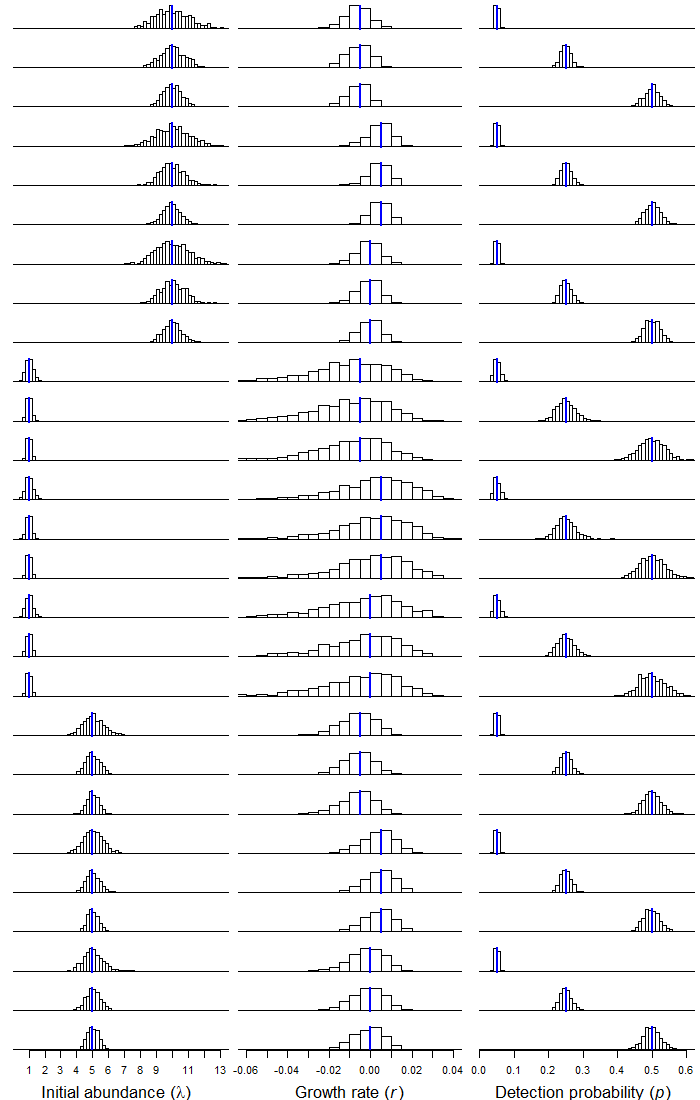
\includegraphics[height=8in]{figs/exp_hists}
  \caption{Histograms of 1000 parameter estimates for each of 27 simulation cases. The verticle lines are the data-generating values.}
\label{fig:exp_hists}
\end{figure}

\section{Discussion}

Our work has highlighted the limitations of classical state-space
models as applied to ecological time series data, and we have
demonstrated how open population $N$-mixture models overcome these
limitations. We extended this class of models in several important
ways, while keeping in mind the practical issues ...

We made four important developments of the open population
N-mixture model proposed by \citep{dail_madsen:2011} that make the
model more applicable to long-term data such as is collected
by the North American Breeding Bird Survey. First, we have
reconciled the objectives of traditional state-space models
with open population $N$-mixture models by illustrating how
classical models of population dynamics can be embedded within
the framework. Second, we have demonstrated methods of
accounting for zero-inflation in the time-series. Third, we
have illustrated how additional random effects such as
observer-specific detection probabilities can be
accommodated. Fourth, we presented a Bayesian analysis of the
model, which, makes it possible to incorporate prior information when
available, and in some cases, facilitates parameter estimation.


A unique aspect of the Dail and Madsen model as originally devised was
that it allowed for the estimation of demographic parameters under
strict distributional assumptions and with the assumption of
geographic closure. Clearly, estimating demographic parameters from
count data is a loftyn ambitious goal, and the required assumption
will not be valid in many cases. Nonetheless, their approach is
important because it allows for the combination of count data with
other data types such as capture-recapture data , which offers a
means of making inferences about demographic processes at broad
spatial scales. Models combining count data and demographic data are
often referred to as integrated population models, and This topic has
received much attention lately under t

In the absence of direct information about demographic parameters, and
when the original assumptions of the model do not hold, we have
offered extensions of the model to estimate derived parameters such as
population growth rate. This has been the traditional emphasis of
state-space models, and our approach resolves many of the factors
limiting ...

[paragraph on zero-inflation]The zero-inflated models for initial
abundance and dynamics allow one to estimate and model the proportion
of sites outside of the range of a species.  This could be especially
useful when different factors control the range than the abundance or
dynamics within the range.  [some examples where that is the case?]

[paragraph on random effects]


[paragraph on Bayesian]
The ability to fit this class of models using freely available MCMC
software offers non-statisticians a powerful means .

In spite of the new extensions we have proposed, several aspects of
the model could be improved. First, the precision with which the
parameters of the state process can be estimated ultimately depends
upon how well detection probability is estimated. When there is only a
single survey per primary period, the information about detection
probability comes from deviations from the parametric assumptions
about population dynamics. Thus, without direct information about
detection probability, the estimates will be determined by model based
assumptions. Furthermore, there are multiple components of detection
probability that should be accounted for to minimize bias and yield
valid estimates of population size \citep{nichols_etal:2009}.

Fortunately, it is easy to incorporate direct information about
detection probability and we recommend that this be done whenever
possible. The original method for proposed in the original paper was
to collected replicated counts within the primary periods during a
period in which the populations could be assumed to be closed.  a
robust design could be used to combine multiple surveys per primary
period to increase the precision of the estimates. We envision that
multiple other options are available as well. For instance, there
should be no difficulty extending the model to accommodate traditional
capture-recapture data collected during each primary period. Removal
or time of detection etc.. Distance-related heterogeneity in detection
probability is another source of variation that can bias estimators of
abundance.   Show some equations for the alternative observation
models.

[paragraph on spatially-explicit dispersal]
[Other possible extensions we could mention:
Spatially hierarchical model (so can use individual stops)
Other models of variability in growth or recruitment (such as negative binomial)
Add density dependence to survival and recruitment models]
[Discuss causes of low p values (and other BBS results) here or in BBS
results?]
Our emphasis was on increasing the practical utility of this class of
models, and so we avoided several conceptually-interesting extensions
that we belive would be computationally prohibitive in many
cases. Nonetheless, we will discuss one---spatially-explict models of
immigration.


The modeling framework we described can be used to address many of the
most pressing issue in ecology and conservation biology. For example,
it is possible to test hypotheses about temporal and spatial
population regulation. Furthermore, the Bayesian approach is very
useful in that it can be used to combine multiple sources of data to
develop mechanistic models of population dynamics. Thus one can test
hypotheses about the effects of climate change on either explicit
demographic parameters or in derived parameters such as population
growth rate. Furthermore, under the Bayesian approach , population
viability analysis is trivial because projecting populations into the
future can be done as a component of the MCMC analysis. This allows
for the computation of posterior distributions of parameters such as
quasi-extinction probability.


\bibliography{Dail_Mad_ext}


\newpage

% Tables


\begin{table}[t]
  \centering
  \caption{Changed parameter values, by series of simulations.  We
    simulated 1000 sets of data each combination of parameter values
    for 100 sites over 40 years.  We assumed that initial abundance
    ($\Lambda$) was Poisson distributed.  For the exponential growth
    simulations we included all combinations of low, medium, and high
    $\Lambda$, growth rate ($r$), and detection probability ($p$).  For the Ricker
    model simulations we used $\Lambda$ = 10 and $p$ = 0.25, and simulated low,
    medium, and high values of $r$ and equilibrium density ($K$).  For the
    Ricker + immigration dynamics model we fixed all parameters the
    same as the Ricker model (with $r$ = 0.05 and $K$ = 10) and simulated
    low, medium, and high values of immigration rate ($\iota$).}
  \begin{tabular}{lcccccccc}
    \hline
    & \multicolumn{3}{c}{Exponential Growth} && Ricker &&
    \multicolumn{2}{c}{Ricker + Immigration} \\
    \cline{2-4}     \cline{6-6}    \cline{8-9}
%    & \multicolumn{3}{c}{\rule{25mm}{.1pt}} & \rule{5cm}{.5pt} & \multicolumn{2}{c}{\rule{20mm}{.1pt}} \\
                & $\Lambda$ & $r$ & $p$ && $r$  && $K$ & $\iota$  \\
    \hline
    Low	        &1	&-0.01	&0.05	&&0.005	&&5	&0.005  \\
    Med	        &5	&0	&0.25	&&0.05	&&10	&0.05   \\
    High	&10	&0.005	&0.5	&&0.1	&&20	&0.5    \\
    \hline
  \end{tabular}
\end{table}

\vfill
%\clearpage
\newpage

% Perhaps stack the species

\begin{sidewaystable}
  \centering
  \small
  \caption{Model selection table for ovenbirds and golden-winged
    warblers in Maryland and Virginia, 1966-2010.  We present model name
    and number, number of parameters (Par.), and difference in Akaike's
    information criterion between each model and the top model of that
    set ($\Delta$AIC).  For each species, the first section compares
    models for initial abundance, the second for detection probability,
    and the third for dynamics.}
  \begin{tabular}[h]{lcclcc}
\hline
A. Ovenbirds	&&&		B. Golden-Winged Warblers \\
\hline
Model	&Par.	&$\Delta$AIC	&Model	&Par.	&$\Delta$AIC \\
A.1. NB[$\Lambda$(.)$\alpha$(.)]Growth[$r$(.)]$p$(.)	&4	&0
&B.1. ZIP[$\Lambda$(.)$\psi$(.)]Growth[$r$(.)]$p$(.)	&4	&0 \\
A.2. P[$\Lambda$(.)]Growth[$r$(.)]$p$(.)	&3	&1262.7
&B.2. NB[$\Lambda$(.)$\alpha$(.)]Growth[$r$(.)]$p$(.)	&4	&0.4 \\
A.3. ZIP[$\Lambda$(.)$\psi$(.)]Growth[$r$(.)]$p$(.)	&4
&1264.7	&B.3. P[$\Lambda$(.)]Growth[$r$(.)]$p$(.)	&3	&37.8 \\
A.4. NB[$\Lambda$(.)$\alpha$(.)]Growth[$r$(.)]$p$(wind+1st)	&8
&0	&B.4. ZIP[$\Lambda$(.)$\psi$(.)]Growth[$r$(.)]$p$(1st)	&5
&0 \\
A.5. NB[$\Lambda$(.)$\alpha$(.)]Growth[$r$(.)]$p$(wind)	&7	&0.9
&B.5. ZIP[$\Lambda$(.)$\psi$(.)]Growth[$r$(.)]$p$(.)	&4	&3.5 \\
A.6. NB[$\Lambda$(.)$\alpha$(.)]Growth[$r$(.)]$p$(1st)	&5	&5.0
&B.6. ZIP[$\Lambda$(.)$\psi$(.)]Growth[$r$(.)]$p$(wind+1st)	&8
&5.9 \\
A.7. NB[$\Lambda$(.)$\alpha$(.)]Growth[$r$(.)]$p$(.)	&4	&6.4
&B.7. ZIP[$\Lambda$(.)$\psi$(.)]Growth[$r$(.)]$p$(wind)	&7	&9.3 \\
A.8. NB[$\Lambda$(.)$\alpha$(.)]Ricker+Imm.[$r$(.)$K$(.)$\iota$(.)]$p$(wind+1st)
&10	&0	&B.8. ZIP[$\Lambda$(.)$\psi$(.)]Growth[$r$(.)]$p$(1st)
&5	&0 \\
A.9. NB[$\Lambda$(.)$\alpha$(.)]Gompertz+Imm.[$r$(.)$K$(.)$\iota$(.)]$p$(wind+1st)
&10	&8.4
&B.9. ZIP[$\Lambda$(.)$\psi$(.)]AR[$\gamma$(.)$\omega$(.)]$p$(1st)
&6	&1.7 \\
A.10. NB[$\Lambda$(.)$\alpha$(.)]Growth+Imm.[$r$(.)$\iota$(.)]$p$(wind+1st)
&9	&36.5
&B.10. ZIP[$\Lambda$(.)$\psi$(.)]Growth+Imm.[$r$(.)$\iota$(.)]$p$(1st)
&6	&2.0 \\
A.11. NB[$\Lambda$(.)$\alpha$(.)]AR+Imm.[$\gamma$(.)$\omega$(.)$\iota$(.)]$p$(wind+1st)
&10	&38.6
&B.11. ZIP[$\Lambda$(.)$\psi$(.)]Gompertz+Imm.[$r$(.)$K$(.)$\iota$(.)]$p$(1st)
&7	&2.6 \\
A.12. NB[$\Lambda$(.)$\alpha$(.)]Gompertz[$r$(.)$K$(.)]$p$(wind+1st)
&9	&190.9
&B.12. ZIP[$\Lambda$(.)$\psi$(.)]Gompertz[$r$(.)$K$(.)]$p$(1st)	&6
&3.0 \\
A.13. NB[$\Lambda$(.)$\alpha$(.)]Ricker[$r$(.)$K$(.)]$p$(wind+1st)
&9	&195.1
&B.13. ZIP[$\Lambda$(.)$\psi$(.)]AR+Imm.[$\gamma$(.)$\omega$(.)$\iota$(.)]$p$(1st)
&7	&3.7 \\
A.14. NB[$\Lambda$(.)$\alpha$(.)]Growth[$r$(.)]$p$(wind+1st)	&8
&271.3
&B.14. ZIP[$\Lambda$(.)$\psi$(.)]Ricker+Imm.[$r$(.)$K$(.)$\iota$(.)]$p$(1st)
&7	&4.2 \\
A.15. NB[$\Lambda$(.)$\alpha$(.)]AR[$\gamma$(.)$\omega$(.)]$p$(wind+1st)
&9	&273.7
&B.15. ZIP[$\Lambda$(.)$\psi$(.)]Ricker[$r$(.)$K$(.)]$p$(1st)	&7
&5.2 \\
A.16. NB[$\Lambda$(.)$\alpha$(.)]Constant[$\gamma$(.)$\omega$(.)]$p$(wind+1st)
&9	&1856.7
&B.16. ZIP[$\Lambda$(.)$\psi$(.)]Constant[$\gamma$(.)$\omega$(.)]$p$(1st)
&6	&12.5 \\
\hline
\end{tabular}
\end{sidewaystable}

\end{document}
